\documentclass{school-22.211-notes}
\date{March 19, 2012}

\begin{document}
\maketitle


\lecture{One-Group Diffusion: Non-Multiplying Medium with No Source} \label{1g-1}

\topic{1D Non-Multiplying Medium With No Source}
\eqn{ \dphidxn2 - \frac{\phi(x)}{L^2} &= 0 }
Assume that flux is in the form of $\phi(x) = C \exp(k x)$, substitute into the differential equation, and it turns out $ k = \pm \frac{1}{L}$. Thus 
\eqn{ \phi(x) = C_1 e^{\frac{x}{L}} + C_2 e^{-\frac{x}{L}} }
We apply BCs: $\phi(0) = \phi_0, \phi(\infty) = $ finite. Thus
\eqn{ \phi(x)  = \phi_0 e^{- \frac{x}{L} } }



\clearpage
\topic{Plane Source in Infinite Non-Multiplying Medium}
Consider an infinite non-multiplying medium with a plane source. We define the coordinate system to start at the source (thus the source is at $x=0$ now), and solve the symmetric problem to avoid having to solve for a general and a particular solution. 

Since the geometry is symmetric, we can solve for $x>0$ first. 
\eqn{ \phi(x) = Ae^{x/L} + B e^{-x/L}} 

BCs: 
\begin{itemize}
\item $\displaystyle \lim_{x \to \infty} \phi(x) = 0, \Rightarrow \phi(x) = B e^{-x/L}$; 
\item $\displaystyle \lim_{x\to 0} J(r)  = \frac{S_0}{2}$. Equate that with $\displaystyle J = -D \dphidx = B D e^{-x/L}$, we get $B = \frac{S_0 L}{2D}$. 
\end{itemize}
\eqn{ \phi(x) = \frac{S_0 L}{2D} e^{-x/L}}
For the total geometry, we can simply place an absolute sign on $x$:
\eqn{ \phi(x) = \frac{S_0 L}{2D} e^{-|x|/L}}
If the source is placed at $x=b$, the solution becomes,
\eqn{ \phi(x) = \frac{S_0 L}{2D} e^{-|x-b|/L} }


\clearpage
\topic{Plane Source in Finite Non-Multiplying Medium}
Consider a finite system from $-a$ to $a$ with vacuum BCs. 

The balance equation is, 
\eqn{ \dphidxn2 - \frac{\Sigma_a}{D} \phi(x) = - \frac{S_0}{D} }
We cannot play the trick in the infinite medium anymore to avoid solving for a homogeneous and a particular solution: 
\eqn{ phi(x) = \phi_{HOM} (x) + \phi_P (x) } 
The homogeneous solution is in the form of exponentials as we have solved for multiply times: 
\eqn{ \phi_H (x) = C_1 e^{ \frac{x}{L}}  + C_2 e^{- \frac{x}{L} } }
Consider the particular solution has to be dependent on the source but independent of the space; that is, 
\eqn{\overbrace{\dphidxn2}^{\to 0} - \frac{\Sigma_a}{D} \phi_P &= - \frac{S_0}{D}  & \phi_P &= \frac{S_0}{\Sigma_a} } 
Putting the homogeneous and particular solution together, and consider vacuum BCs on the extrapolated boundaries $\pm \tilde{a} = \pm (a + 2D)$: 
\begin{itemize}
\item $\phi(\tilde{a}) = 0$. 
\item $\phi(-\tilde{a}) = 0$. 
\end{itemize}
We get to, 
\eqn{ C_1 = C_2 = - \frac{1}{ e^{\frac{\tilde{a}}{L}} + e^{-\frac{\tilde{a}}{L}} } \frac{S_0}{\Sigma_a} }
Then we write our final solution in $\sinh, \cosh$, 
\eqn{ \phi(x) = \left( 1 - \frac{\cosh \left( \frac{x}{L} \right)}{\sinh \left( \frac{x}{L} \right)} \right) \frac{S_0}{\Sigma_a} }


\clearpage
\topic{Point Source in Infinite Non-Multiplying Medium}
Conside an infinite non-multiplying medium with a point source. Eq.~\ref{bal-eqn} become,
\eqn{ \dphidrn2 + \frac{2}{r} \dphidr - \ols\phi = -\frac{S_0}{D} \delta(\vecr) }
We look for the homogeneous solution, and set \hi{$w = r \phi$} (this is an important trick because it would make a spherical case identical to the plane case), 
\eqn{ \dphidrn2 + \frac{2}{r} \dphidr - \ols\phi &= 0, &\dwdrn2 - \ols w &= 0}
The solution is, 
\eqn{ w &= Ae^{r/L} + B e^{-r/L}, & \phi(r) = A\frac{e^{r/L}}{r} + B \frac{e^{-r/L}}{r} }

BCs: 
\begin{itemize}
\item $\displaystyle \lim_{r\to \infty} \phi = 0, \Rightarrow A=0$.
\item $\displaystyle  \lim_{r\to 0} 4 \pi r^2 J(r) = S_0$ (this is also the particular solution), that is, 
\begin{align}
J &= -D \dphidr = DBe^{-r/L} \left( \frac{1}{r^2} + \frac{1}{rL} \right)
&\lim_{r\to 0} 4 \pi r^2 J(r) &= 4 \pi DB = S_0 &B &= \frac{S_0}{4 \pi D}
\end{align}
\end{itemize}
\eqn{\Aboxed{ \phi(r) &= \frac{S_0}{4\pi D} \frac{e^{-r/L}}{r}  } }

Interpretations:
\begin{enumerate}
\item Extreme condition 1: no absorption: as $\Sigma_a \to 0, L\to \infty$, 
  \eqn{\lim_{L\to \infty} \phi(r) = \frac{S_0}{4 \pi Dr}  = \mbox{Geometrical Attenuation}}
\item Extreme condition 2: pure absorber. We can easily solve the transport kernel: 
  \eqn{\phi(r) = \int_{V'} \frac{S(r') e^{-\Sigma_a|r-r'|}}{4\pi|r-r'|^2}  = \frac{S_0}{4 \pi r^2} }
\item Diffusion results in a different shape for the decrease in neutron population as in Figure~\ref{dfs-shape}.
  \begin{figure}
    \centering
    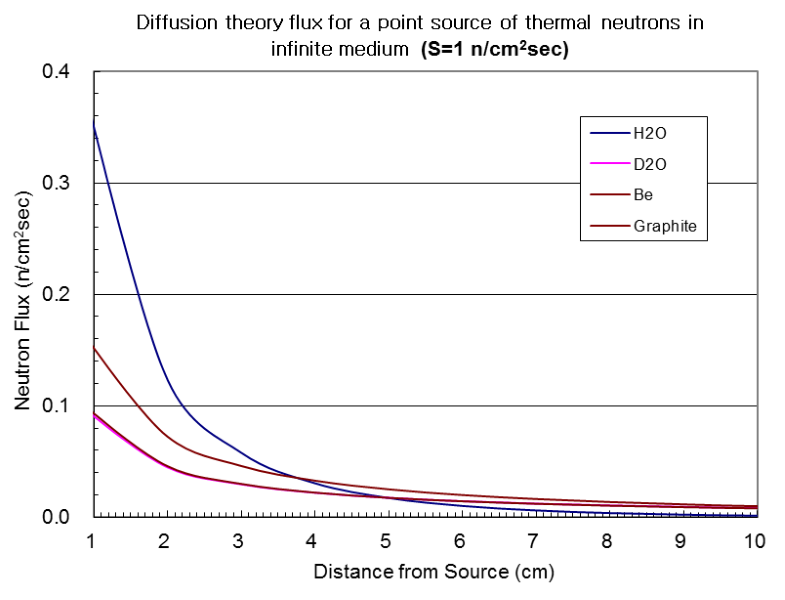
\includegraphics[width=4in]{images/dfs/dfs-shape.png}
    \caption{Flux Shape Depent On Diffusion Coefficients}\label{dfs-shape}
  \end{figure}
\item At $r=0$ tere is a non-physical singularity due to the mathematical artifact of point sources;
\item Diffusion theory is not valid near singularities;
\item We can use diffusion kernel to solve source problems in non-multiplying media by superposition.
\end{enumerate}




\end{document}
